\subsubsection{Общая структура проектного решения}
Глобально проект состоит из двух компонент. Первая отвечает за интерактивное
взаимодействие с пользователем и генерацию кода второй компоненты с
использованием указанных пользователем алгоритмов (далее --- компоновщик).
Вторая --- это имплементация блокчейна (далее --- реализация блокчейна).
Проект содержит код для кошелька ({\small wallet.py}) и майнера ({\small
miner.py}) с определённой функциональностью. Код второго проекта структурирован
для удовлетворения нужд использования указанных пользователем методов. Методы и
классы генерируются at-runtime первого приложения.

\begin{itemize}
    \item Язык программирования --- Python версии 3.6.5
    \item Тип: консольная утилита
    \item Протокол обмена данными между компонентами: http + json
    \item База данных: key-value хранилище
    \item Запуск скриптов обновления: UNIX cron
    \item Continuous integration: Shippable
    \item License: GNU GPL v3
    \item Конфиг: YAML
\end{itemize}

\subsubsection{Архитектура компоновщика}
Компоновщик --- часть проекта, автоматизирующая процесс программирования и
позволяющяя тем самым создавать готовые решения. Решением может быть рабочий
код блокчейна с использованием 24 вариаций алгоритмов.
\subsubsection{Порядок работы компоновщика}
Программно компоновщик был назван {\small gsl}. Основная команда с которой
придётся иметь дело --- init. Пример:\\

\begin{center}
    {\small gsl --init --name myledger --path ~/tmp/gsl}
\end{center}

\begin{figure}[h]
    \centering
    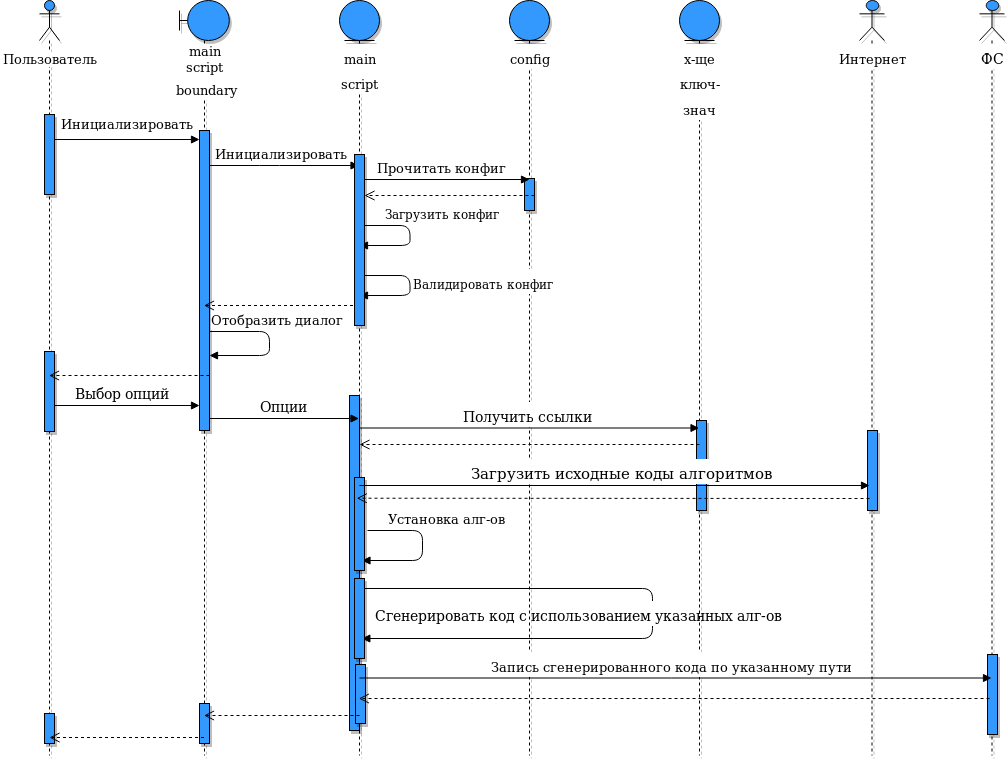
\includegraphics[width=\textwidth]{images/sequence}
    \caption{Sequence диаграмма последовательности работы первой компоненты}\label{sequence}
\end{figure}

\newpage
По вызову этой команды происходят процессы, обозначенные на диаграмме
последовательностей (Рис.  \ref{sequence}). Зачитывается, загружается в
программу и валидируется конфигурационный файл программы.

\newpage

Затем начинается диалог с пользователем (Рис. \ref{dialog}).
\begin{figure}
    \centering
    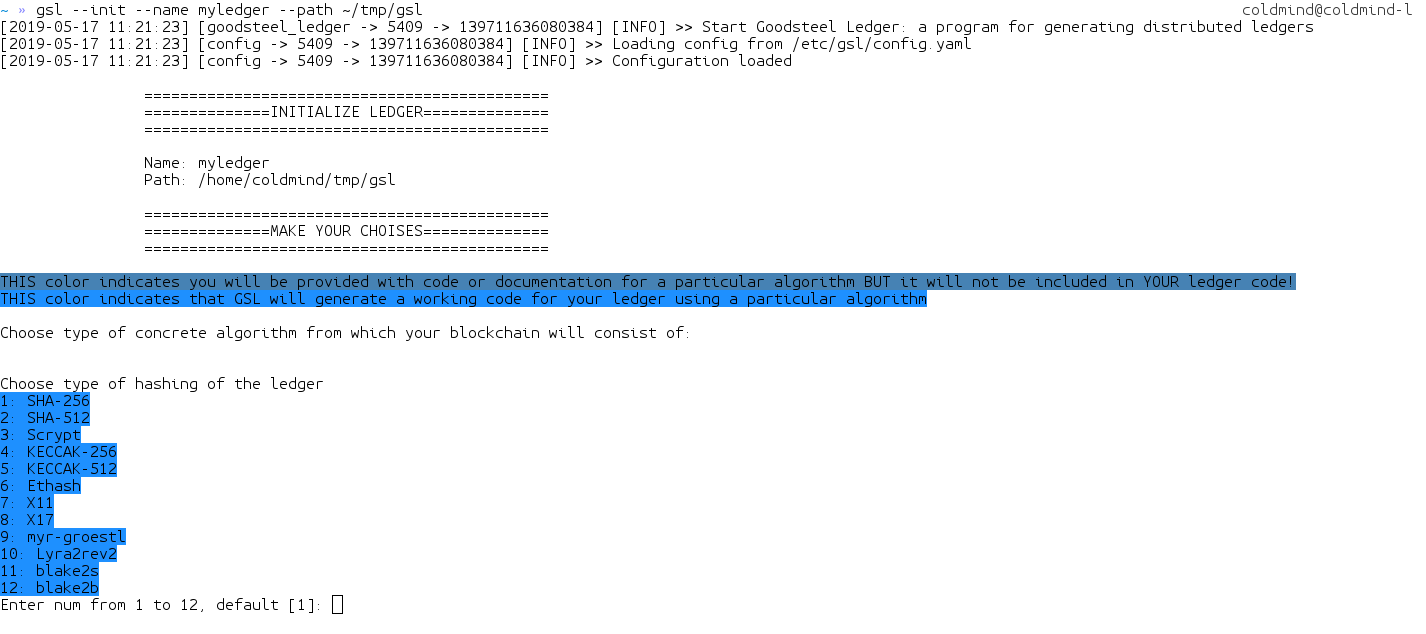
\includegraphics[width=\textwidth]{images/dialog_start}
    \caption{Начало диалога выбора алгоритмов}\label{dialog}
\end{figure}

В этом диалоге пользователь выбирает какие алгоритмы хэширования и цифровой
подписи будут использованы в его будущей реализации блокчейна. После этого,
пользователю предоставляется выбор других интересных параметров блокчейна, по
которым ему будут предложены справочные ссылки для изучения (Рис. \ref{sprav}).
После выбора происходит установка данных библиотек и генерация кода реализации
блокчейна по указанному пути (Рис. \ref{ll}).

\begin{figure}[h]
    \centering
    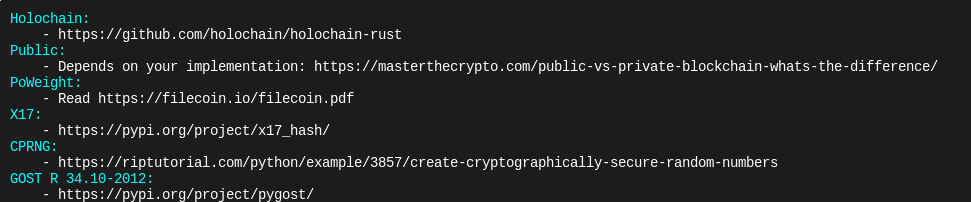
\includegraphics[width=\textwidth]{images/spravochno}
    \caption{Справочная информация по выбранным параметрам}\label{sprav}
\end{figure}

\subsubsection{Архитектура реализации блокчейна}
\begin{figure}[h]
    \centering
    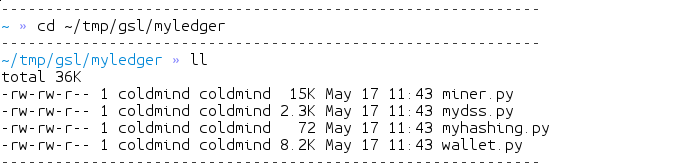
\includegraphics[width=0.8\textwidth]{images/ledger_ll}
    \caption{Директория со сгенерированным кодом реализации блокчейна}\label{ll}
\end{figure}

Код реализации блокчейна запускается интерпретатором языка Python 3.6.5.
Скрипты {\small miner.py} и {\small wallet.py} запускаются без аргументов
командной строки. Запустив {\small miner.py} (Рис. \ref{miner_run}), можно запускать {\small
wallet.py} (Рис. \ref{wallet_run}), в котором есть возможности:
\begin{enumerate}
    \item Сгенерировать кошелёк: пару публичный-приватный ключи и записать их в файл
    \item Отправить с одного кошелька на другой N условных едениц
    \item Провалидировать транзакции
\end{enumerate}

\begin{figure}[h]
    \centering
    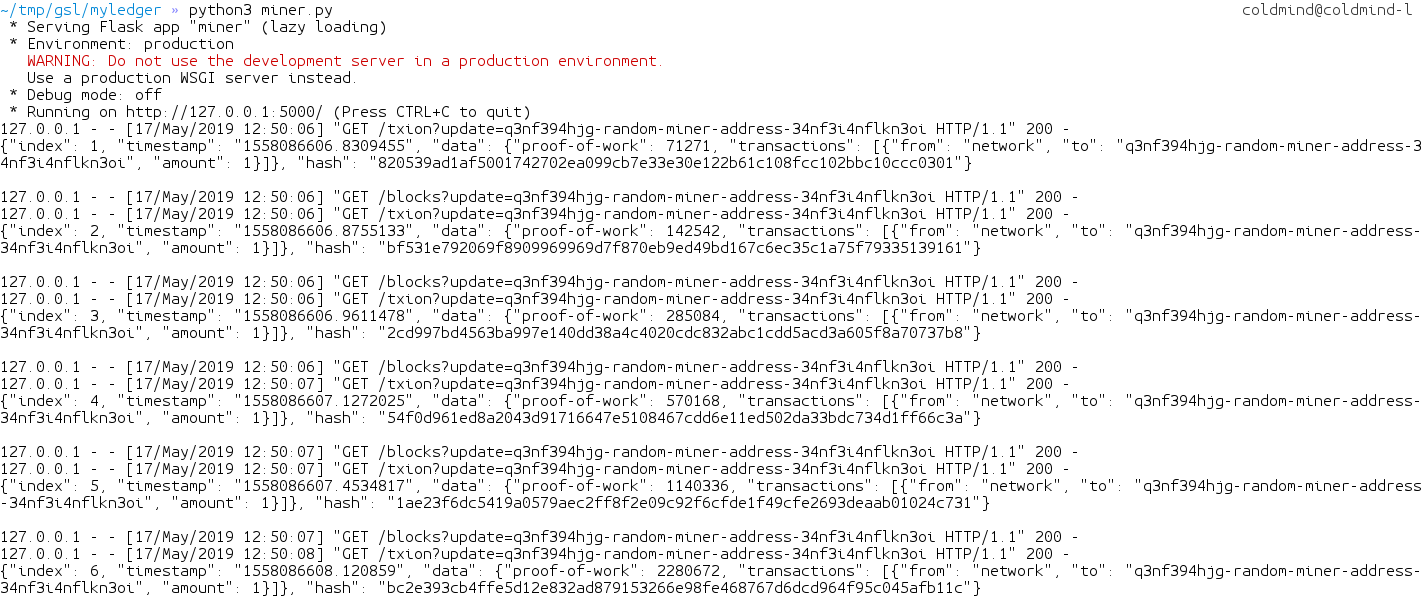
\includegraphics[width=\textwidth]{images/miner_run}
    \caption{Лог запуска майнера}\label{miner_run}
\end{figure}

\begin{figure}[h]
    \centering
    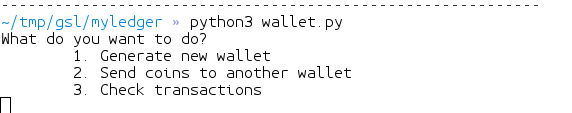
\includegraphics[width=0.8\textwidth]{images/wallet_run}
    \caption{Возможности кошелька}\label{wallet_run}
\end{figure}

Генерация пары ключей, а так же хэширование записей происходит посредством
использования выбранных ранее пользователем алгоритмов.:w

\subsubsection{Работа с данными}
Исходный код алгоритмов хранится в директории {\small src/altorithms/hashing} и
{\small src/altorithms/digital\_signature}. Он собирается полным проходом в
сеть по ссылкам, расположенными в импровизированном key-value хранилище
(описано в настоящем техническом задании --- Приложение ref1). Данная процедура
происходит при автообновлении алгоритмов на сервере каждый день в 21:00
(Рис. \ref{update}). После процедуры автообновления, пользователи могут по
желанию обновить свою версию программы и использовать более свежий код.

\begin{figure}[h]
    \centering
    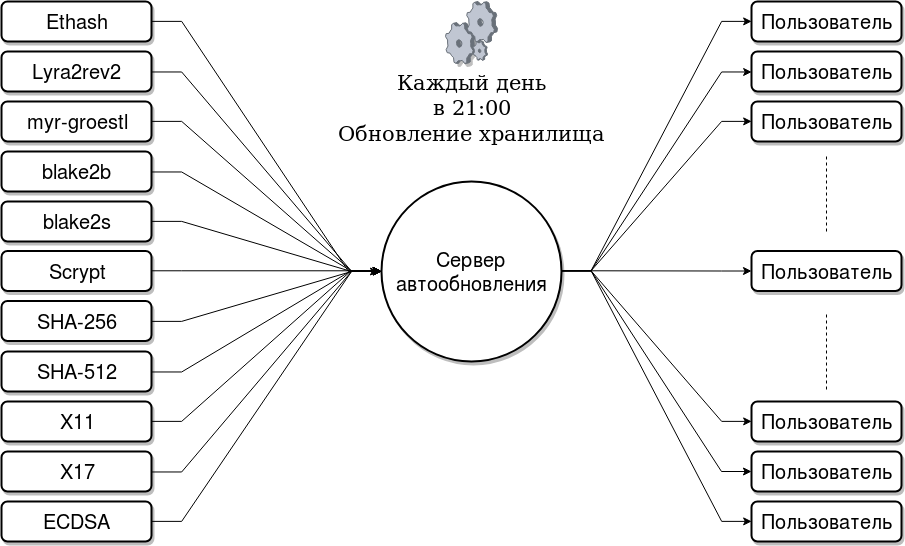
\includegraphics[width=\textwidth]{images/server}
    \caption{Процесс работы сервера автообновления}\label{update}
\end{figure}


\subsubsection{Язык программирования}
Выбор пал
